\chapter{Methods}
\label{chapter:methods}
One approach for estimating energy consumption of a given network is by employing actual power meter to measure the power drawn by involved network and computing components. A good example for such case is the measurement that Fan and his team conducted\cite{DBLP:conf/isca/FanWB07}. In this study the authors have managed to monitor power consumption of several thousand of servers over a period of six months on real live workload. Mahadevan et al.{\ } have also done a similar power measurement on a production environment for studying power consumption behavior of networking devices such as switches and routers. If the measurements are done correctly, this approach produces the most real picture of the network under investigation compared to the other approaches discussed in subsequent paragraphs. However, this approach has certain inherent drawbacks. First real production networks might not be available for experimentation. Even if they become available, the transient and varying nature of the production environment makes it hard to repeat the experiment. Second we have little or no control over factors affecting the measured power consumption. We do not have the privileged of injecting or modifying the traffic or the workload in order to test different experimental hypothesis. To have a full control we need another approach. That is what we discuss next.

Experimental testbed is another approach that researchers have used to study power consumption characteristics of different computing and networking equipments. In this approach first a separate network is setup and configured solely for the purpose of conducting experiments. Then researchers make measurements by manipulating factors that affect power consumption according to the hypothesis that they want to test. Unlike the previous one, this approach offers greater flexibility over the experimental parameters. In the power measurement study scenario that we are discussing, the researcher can change parameters such as traffic rate, packet size, inter-packet time interval and transmission protocol used (TCP/UDP). Sivaraman et al.{\ } in \cite{Sivaraman} have setup experimental testbed for determining per-packet processing and per-byte receipt, storage, queuing, and transmission power consumption. The experiment setup involved hardware-based traffic generator (which gives fine grain control over parameters such as the packet size, inter-packet interval and data rate), NetFPGA\footnote{http://www.netfpga.org/} experimental router and digital oscilloscope for measuring the power draw of the NetFPGA router. A similar experiment but with a commercial switches of different vendors is explained in \cite{DBLP:journals/comcom/SivaramanRZSVMR14}. The primary advantages of this approach is that the researcher can have full control over the experimental parameters provided by the tools involved in the testbed and experimental result can also be very accurate. The first disadvantage though is that it can easily become very expensive when we want to experiment on large-scale level. The second disadvantage is that experimenting on different scenario might require considerable reconfiguration and even a completely new testbed, which apart from limiting the flexibility, it can also be very costly, time and effort consuming. We need an approach which overcome these shortcomings. That is, we need an approach which gives full control over the experiment, which is reasonably accurate, less expensive and very flexible. 

Simulation is the most widely used approach in computer network researches \cite{DBLP:conf/icc/WeingartnerLW09}. It has several advantage compared to the other two approaches mentioned before. First it is relatively easy to study, for instance, the performance of non-existing network protocol or algorithm using simulator. To give an example one can propose and validate, by simulation experiment, a new energy-aware routing protocol or algorithm for wired or wireless networks. This is exactly what Swain et al.{\ }\cite{DBLP:conf/aina/SwainHC10} did in their new energy-aware routing protocol proposal for wireless sensor networks. Second, though it depend on the design of the particular simulator used, in general, simulation approach allows running large scale experiments that involve hundreds and thousands of nodes compared to the other two approaches. In \cite{DBLP:conf/wowmom/OrgerieLLL11} and \cite{DBLP:conf/cloudnet/CorneaOL14}, ECOFEN - the NS-3 module is used to simulate energy consumption of large-scale networks with nodes more than 600 and 1000, respectively. In \cite{DBLP:journals/tjs/KliazovichBK12}, the authors studied energy consumption of data center networks with two-tier and three-tire architectures that encompasses 1536 nodes. Third, in simulation scaling does not incur monetary cost, rather, it is limited by performance factors such as runtime and memory usage \cite{DBLP:conf/icc/WeingartnerLW09}. Fourth, the researcher has great flexibility and full control over the simulation experiment. 

Though simulation experiment has quite a lot of advantages over experiments done on production environment or experimental testbeds, it faces one big challenge, accuracy. In the process of approximating the real network phenomenon in the simulation model, some less significant concepts are abstracted away, for instance, to reduce complexity or to gain performance improvement, which results in unavoidable loss of accuracy. However, in other instances the models used in a given simulator might fail to correctly capture the simulated real network phenomenon. In \cite{DBLP:journals/tomacs/VelhoSCL13} the authors demonstrated incorrect modelings found in popular simulators such as OptorSim, GridSim and CloudSim. Therefore, (in)validating the correctness of a simulator is important task that should be undertaken before any simulation experiment for two related reasons. Either to know the boundaries within which the simulator used produce reasonably accurate results, or to know if the simulator produce the expected or the correct result. The validation can be done either by comparing the output of the simulator against accurate measurements obtained from real networks or by comparing the output against another simulator whose accuracy is already known\cite{DBLP:books/daglib/0076234}.
\section{Our Approach}
\label{section:ourapproach}
The purpose of this study is to implement analytical or flow-level (as opposed to packet-level) energy consumption model for SimGrid and to show that the implemented model produce reasonably accurate result and is also scalable for estimating energy consumption of large-scale distributed networks. To achieve this goal, we use the simulation approach among the three alternatives discussed above. 

Before describing the details of our approach, let us first justify why we end up with the relatively complex method shown in Figure~\ref{fig:approach}. There is experimental test-bed (Grid5000\footnote{https://www.grid5000.fr/mediawiki/index.php/Grid5000:Home}) in France that we have access to. Grid5000 is experimental test-bed specifically designed for studying large-scale distributed networks \cite{DBLP:journals/ijhpca/BolzeCCDDJJLLMMNPQRTT06}. However, we could not used it for our purpose (i.e., for studying large-scale flow-level relationship of power consumption and traffic) as the nodes are not equipped with tools such as traffic generator and power meter. As a result, we opted to use a packet-level simulator with power consumption models obtained from literature. Subsequent paragraphs describe the specific tasks we performed in relation to this approach.

As we have discussed in Chapter~\ref{chapter:background}, SimGrid already have energy consumption model for CPU which corresponds to the computing part of a given large-scale network. What we wanted to add is energy consumption model for communication components such as switches and routers. Therefore, the initial task in our approach is to study literatures (\circled{1} in Figure~\ref{fig:approach}) in order to find a model which describe the power consumption characteristics of communication equipments such as switches and routers. Our search returned the linear relationship that we have described in Equation~\ref{eq:2.2} \cite{Sivaraman,DBLP:journals/comcom/BeisterDAK14,DBLP:conf/networking/MahadevanSBR09,DBLP:conf/sigcomm/MahadevanBS10}. This equation tells us that the power consumption of a network equipment constitutes the idle and dynamic components. The idle power consumption represents the power drawn by the equipment while it is on but with no traffic. The dynamic consumption, on the other hand, represent the additional power drawn due to network traffic. The next task (\circled{3} in Figure~\ref{fig:approach}) is to implement this linear model for SimGrid and (in)validate its accuracy against ECOFEN module (\circled{4} in Figure~\ref{fig:approach})\cite{DBLP:conf/wowmom/OrgerieLLL11,DBLP:conf/cloudnet/CorneaOL14}. The final task (\circled{7} in Figure~\ref{fig:approach}) is to show the scalability of the implemented flow-level model against the existing packet-level model in ECOFEN. For this we design and run two kinds of experiments (\circled{5} and \circled{6} in Figure~\ref{fig:approach}), one for speed and one for memory usage. 

We chose to use ECOFEN as packet-level simulator to compare the accuracy and performance of the implemented model for two primary limitations apparent in the other alternative simulator, GreenCloud \cite{DBLP:journals/tjs/KliazovichBK12}. The first limitation is that GreenCloud is designed for cloud computing environment. This is in contrary to one of SimGrid's main designed principle, versatility \cite{DBLP:journals/jpdc/CasanovaGLQS14}. ECOFEN, on the other hand, is not tied to one particular large-scale networking paradigm, therefore, suits more for our purpose. The second limitation of GreenCloud is that it is build on top of currently obsolete NS-2 simulator. In comparison, though ECOFEN was also initially built as NS-2 simulator module, currently it is rewritten for NS-3 \cite{DBLP:conf/cloudnet/CorneaOL14}. One of the major advantage of using NS-3 over NS-2 is that NS-3 performs considerably well in both runtime and memory-usage metrics \cite{DBLP:conf/icc/WeingartnerLW09}.

In the accuracy-validation and scalability-comparison experiments mentioned in our approach, we are comparing the newly implemented flow-level model in SimGrid simulator against another packet-level simulator model implemented in ECOFEN module. This simulator-to-simulator comparison is valid only if the later simulator model, against which the new implementation is to be validated, is known to be accurate. However, we could not find any information that tell us the accuracy of the ECOFEN module. Therefore, we designed a validation experiment (\circled{2} in Figure~\ref{fig:approach}) for ECOFEN as described in the next section. 

\begin{figure}[ht]
	\begin{center}
		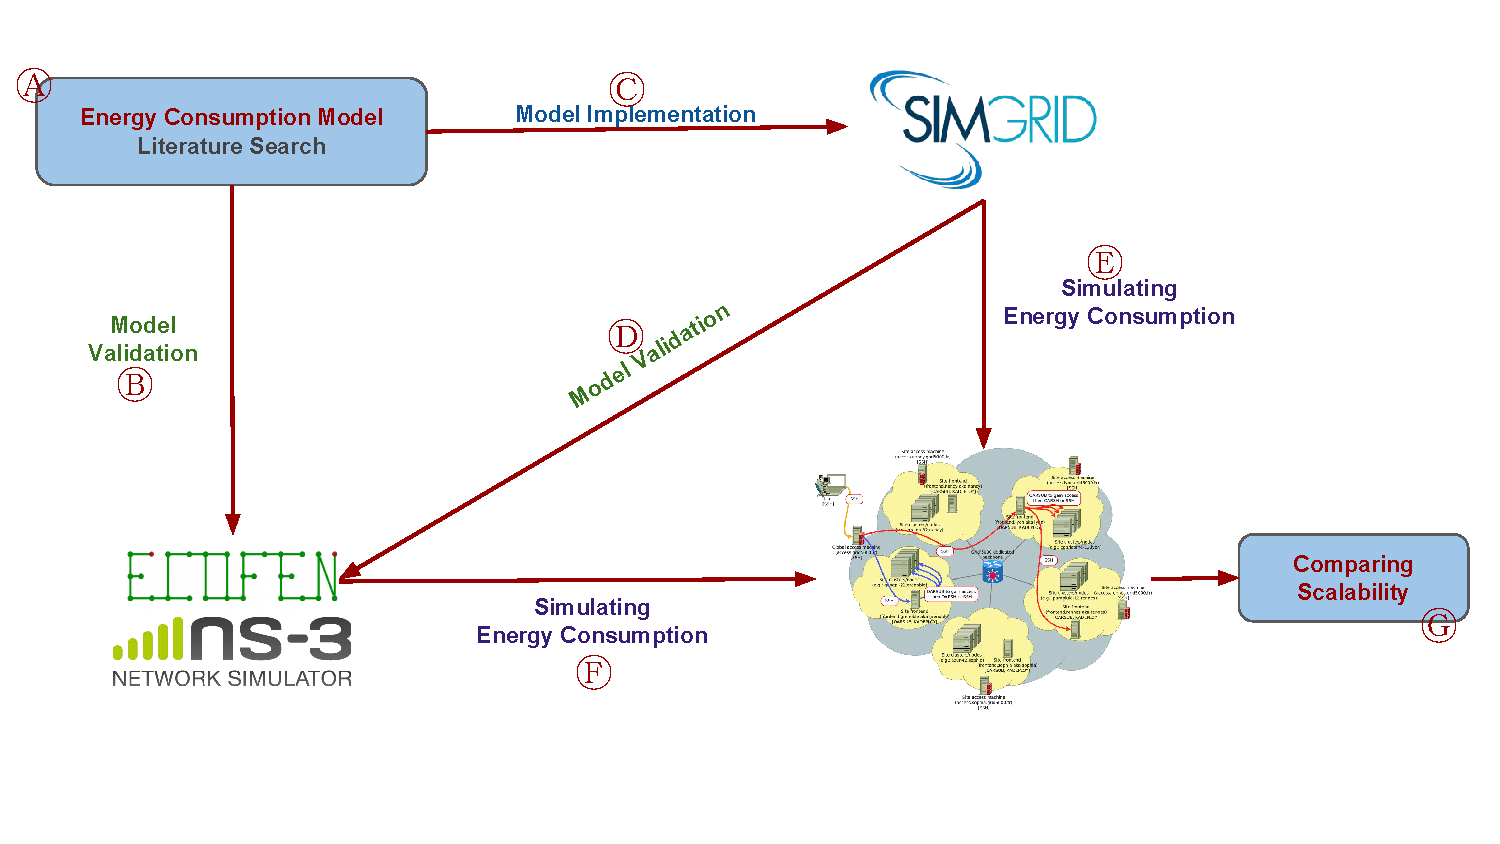
\includegraphics[width=16cm]{images/approach.pdf}
		\caption{Summary of the method we followed in this study}
		\label{fig:approach}
	\end{center}
\end{figure}
\section{Validating ECOFEN}
 ECOFEN has three models with names \emph{basic}, \emph{linear} and \emph{complete} that we have discussed in Section~\ref{section:relatedsimulator} of Chapter~\ref{chapter:background}. The \emph{linear} and \emph{complete} models